\subsubsection{Users}
\def\arraystretch{2}
\begin{table}[H]
\centering
\begin{tabular}{|l|l|}
\hline
Model & User \\ \hline
Controller & UsersControllers \\ \hline
View & Users \\ \hline
Requisiti & ROP 14, ROP 15, ROP 16, RFP 18, ROO 19, ROO 20, ROO 21 \\ \hline
\end{tabular}
\caption{Tracciamento componente-requisiti Users}
\end{table}
Questa componente si occupa della gestione degli utenti, dagli amministratori di OSS agli operatori e con l'estensione di OSS si andrà ad aggiungere anche il personale delle strutture.
Dato che il sistema OSS verrà reso accessibile anche all'esterno della rete \net, si è obbligati a rispettare le direttive sulla privacy, per questo sono stati aggiunti il campo email e il campo approvato nella relativa tabella del database  e la possibilità di recuperare autonomamente la password persa. Vi è inoltre l'obbligo di modificare la password ogni sei mesi in quanto il sistema contiene \glossario{dati personali} (Ma non \glossario{dati sensibili}).
Quest'ultima funzionalità è già implementata.

\begin{table}[H]
\centering
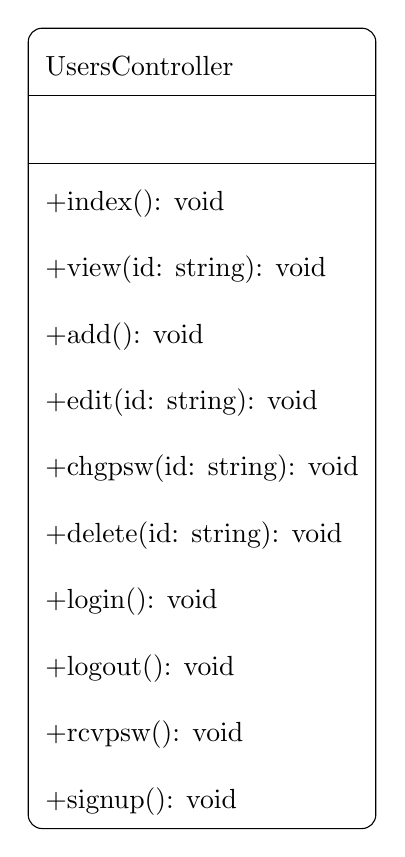
\begin{tikzpicture}
\node (table) [inner sep=0pt] {
\begin{tabular}{l}
  {UsersController} \\
  \hline
  \\
  \hline
  +index(): void \\
  +view(id: string): void  \\
  +add(): void \\
  +edit(id: string): void \\
  +chgpsw(id: string): void \\
  +delete(id: string): void \\
  +login(): void \\
  +logout(): void \\
  +rcvpsw(): void  \\
  +signup(): void  \\
\end{tabular}
};
\draw [rounded corners=.5em] (table.north west) rectangle (table.south east);
\end{tikzpicture}
\caption{Controller:UsersController}
\end{table}



\paragraph{Login}

Il processo di autenticazione esiste già, devono però essere apportate le seguenti modifiche:
\begin{itemize}
\item Nella view va aggiunto un link per il recupero password, che chiamerà il metodo rcvpsw e uno per la registrazione che chiamerà il metodo signup;
\item L'autenticazione dovrà verificare oltre alla corrispondenza username/password anche se tale utente è attivo, controllando se il flag "approvato" è impostato a 1. Questo è possibile farlo aggiungendo l'elemento scope all'array che imposta le opzioni del componente Auth in AppController.php.
\end{itemize}

\label{hash} CakePHP offre la crittazione tramite hash con algoritmo \glossario{MD5}, SHA1, \glossario{SHA256} e blowfish. Attualmete viene utilizzato SHA1. Va tenuto presente però che al momento OSS è un software interno mentre dopo l'espansione verrà reso accessibile anche all'esterno. Per tale motivo il tirocinante suggerisce di passare ad una crittazione più forte come SHA-256, comunque supportata nativamente da CakePHP.

\paragrafo{Diagramma delle attività}

Di seguito è presentato il diagramma delle attività riguardante l'autenticazione a OSS. I soggetti di tali azioni sono operatori e personale.\\

\begin{figure}[H]
\centering
\includegraphics[width=0.8\textwidth]{images/user_login.png}
\caption{Diagramma attività: Login}
\end{figure}

\paragraph{Recupero password}

Il sistema non prevede la possibilità di recupero password, si tratta quindi di una nuova funzionalità. Quando l'utente richiede di recuperare la password:
\begin{itemize}
\item Il sistema genera una passoword casuale di 8 caratteri;
\item Il sistema cripta la passowrd generata con l'algoritmo scelto e salva l'output nel campo password relativo all'utente;
\item Il sistema invia una email con la password all'utente;
\item Nel frattempo l'utente è stato reindirizzato alla pagina di login dove un'avviso gli comunica di controllare la propria casella email;
\item L'utente utilizza la password ricevuta per autenticarsi.
\end{itemize} 

\paragrafo{Diagramma delle attività}
Di seguito è presentato il diagramma delle attività riguardante il recupero password. I soggetti di tali azioni sono operatori e personale.\\


\begin{figure}[H]
\centering
\includegraphics[width=0.6\textwidth]{images/user_rcvpsw.png}
\caption{Diagramma attività: Recupero password}
\end{figure}


\paragraph{Nuovo utente}
Al momento all'interno di OSS sono presente solamente alcuni operatori. Dato che anche il personale delle strutture utilizzerà OSS è necessario che essi possano registrarsi. Non è indicato che sia l'amministratore ad inserirli a sistema in quanto il sistema contiene \glossario{dati sensibili} e dunque la password deve essere conosciuta solo dal proprietario del profilo.

\paragrafo{Diagramma delle attività}
Di seguito è presentato il diagramma delle attività riguardante la creazione di un nuovo utente. I soggetti di tali azioni sono personale e l'amministratore di OSS.\\

\begin{figure}[H]
\centering
\includegraphics[width=0.6\textwidth]{images/user_new_user.png}
\caption{Diagramma attività: Creazione nuovo account}
\end{figure}


\paragraph{Mokup View}
Di seguito un mockup dell'interfaccia utente per la creazione di un nuovo utente.
I mockup di tutti gli altri casi non vengono creati in quanto banali.
\begin{figure}[H]
\centering
\includegraphics[width=0.3\textwidth]{images/mockup_nuovo_utente.png}
\caption{Mockup nuovo utente}
\end{figure}


\subsubsection{Tdocumentos}\label{tdocumentos}
\def\arraystretch{2}
\begin{table}[H]
\centering
\begin{tabular}{|l|l|}
\hline
Model & Tdocumento \\ \hline
Controller & TdocumentosControllers \\ \hline
View & Tdocumentos \\ \hline
Requisiti & ROU 2, ROU 3, ROU 4, ROU 5, RFU 12, ROO 23, ROO 24, ROS 26 \\ \hline
\end{tabular}
\caption{Tracciamento componente-requisiti Tdocumentos}
\end{table}

\begin{table}[H]
\centering
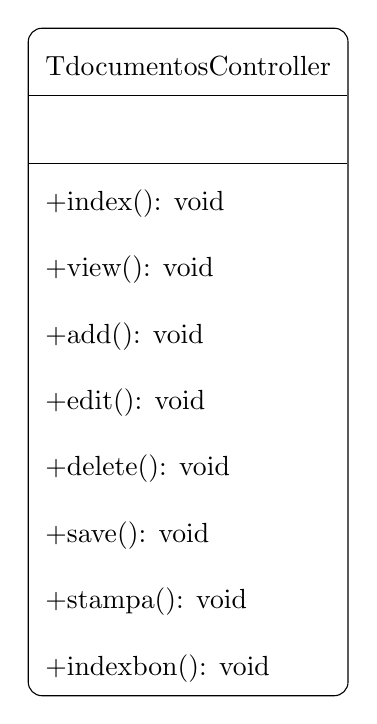
\begin{tikzpicture}
\node (table) [inner sep=0pt] {
\begin{tabular}{l}
  {TdocumentosController} \\
  \hline
  \\
  \hline
  +index(): void \\
  +view(): void \\
  +add(): void \\
  +edit(): void \\
  +delete(): void \\
  +save(): void \\
  +stampa(): void \\
  +indexbon(): void\\
\end{tabular}
};
\draw [rounded corners=.5em] (table.north west) rectangle (table.south east);
\end{tikzpicture}
\caption{Controller:TdocumentosController}
\end{table}


La vendita di un qualsiasi articolo, PadovaCard compresa, al momento inizia da questo controller, con la creazione di un nuovo documento e l'associazione dell'anagrafica di un cliente. \\

Di seguito viene descritto il processo di vendita della PadovaCard attuale:
\begin{itemize}
\item L'operatore seleziona "Nuovo Documento";
\item L'operatore seleziona un anagrafica cliente, o la crea se non esiste;
\item L'operatore sceglie quale PadovaCard vendere;
\item La vendita si conclude con il pagamento.
\end{itemize}
Mentre con il nuovo sistema il processo di vendità diventerà:
\begin{itemize}
\item Da \tlite viene generato un file di testo, come descritto nella Sezione \ref{progettazionetlite};
\item L'operatore seleziona "Nuovo Documento";
\item L'operatore seleziona un anagrafica cliente, o la crea se non esiste;
\item Il file di testo \tlite corrispondente viene caricato;
\item Il sistema ne estrae i seguenti dati:
	\begin{itemize}
        \item Codice operatore;
        \item Codice cassa;
        \item Codice \tlite;
        \item Elenco di data e ora delle varie visite.
	\end{itemize}
\item L'operatore associa ad ogni visita un pacchetto, un nominativo e una data/ora di inizio validità;
\item Il sistema verifica che tale data comprenda al suo interno la visita alla \cappella;
\item L'operatore visualizza il totale e lo comunica al cliente che decide il metodo di pagamento;
\item Con carta di credito la vendita viene conclusa e il sistema invia all'utente inserito su \tlite una mail contenente i voucher e tutti i dati necessari.
\item Con bonifico bancario il sistema invierà una email all'utente specificando i dati per il versamento, quindi a pagamento effettuato\footnote{Gli operatori controllano quotidianamente gli estratti conto del conto corrente} la carta viene spuntata come attiva.
\end{itemize}

\paragrafo{Diagrammi delle attività}

Di seguito è presentato il diagramma delle attività riguardante il processo di vendita di una PadovaCard. 
\begin{figure}[H]
\centering
\includegraphics[width=0.6\textwidth]{images/tdocumentos.png}
\caption{Processo di vendita su OSS}
\end{figure}

\paragraph{Caricamento del file testuale}

Vi sono due possibilità, caricamento manuale o automatico.\\
Con il caricamento manuale è l'operatore che dopo aver cliccato su "Nuova Padova Card" dovrà cliccare su "Carica File" quindi selezionare il file corretto.
Il sistema controllerà che la data di creazione del file non sia troppo precedente alla data di apertura (10 minuti). \\

Con il caricamento automatico l'operatore clicca su "Nuova Padova Card" e quindi su "Carica File" ma è OSS che accede alla cratella in cui si trovano i file, carica tutti i files presenti quindi carica i dati del file di proprietà dell'operatore\footnote{All'interno del file c'è sia il codice operatore che il codice cassa, che sarà confrontato con la login di OSS.}. Una volta caricati i dati su OSS il file viene spostato in una cartella diversa che sarà utilizzata come storico.\\ 

In entrambi i casi è possibile non caricare nessun file, se non vi è nessuna prenotazione da associare, cliccando sul tasto "avanti". \\

Si è deciso di utilizzare il caricamento automatico.

\paragraph{Come vengono estratti i dati dal file} 
Per informazioni sul funzionamento del parser vedere la Sezione \ref{parser}.
Il parser ritornerà le informazioni organizzate in un array di questo tipo:
\begin{lstlisting}
array(
	(int) 0 => array(
		'tlite' => 'TLITE0528719557735',
		'data' => '14/05/2015',
		'ora' => '17:15',
		'numero' => '1'
	),
	(int) 1 => array(
		'tlite' => 'TLITE0528719557740',
		'data' => '14/05/2015',
		'ora' => '17:30',
		'numero' => '2'
	)
)
\end{lstlisting}

\paragraph{Funzionamento del pagamento} 
\paragrafo{Contanti} Il pagamento in contanti prevede un'interfaccia con una semplice calcolatrice per il resto.
\paragrafo{Carta di credito} OSS, cosi come altri gestionali sviluppati da \net utilizza una procedura scritta in PHP che si occupa della creazione di una connessione sicura ai circuiti bancari per il pagamento con carta di credito. Tale procedura è separata dal resto del codice, e non verrà modificata. L'interfaccia prevede il form creato da tale procedura e un link per concludere la vendita.
\paragrafo{Bonifico} Oss rende disponibile un link per inviare al cliente una mail con i dati per il bonifico. Dopo aver inviato la mail è possibile concludere il pagamento. \'E compito degli operatori verificare l'estratto conto, al di fuori di OSS per verificare se il cliente ha versato la somma corretta.

\paragraph{Informazioni in possesso dell'utente al termine del processo} 

L'utente la cui anagrafica è stata inserita a livello di documento è l'unico di cui si conosce l'email, pertanto sarà lui il destinatario della mail contenente le informazioni. Tale mail la cui veste grafica è visible nell'Appendice %TODO 
conterrà le seguenti informazioni:
\begin{itemize}
\item Anagrafica del cliente;
\item Numero di PadovaCard acquistate;
\item Totale pagato;
\item I voucher di ogni PadovaCard, ognuno composto da:
	\begin{itemize}
		\item Codice a barre della PadovaCard;
        \item Codice a barre di \tlite (Se presente);
        \item Strutture visitabili con il pacchetto scelto;
        \item Data e ora della visita alla \cappella (Se presente).
	\end{itemize}
\end{itemize}

\paragraph{Informazioni in possesso del sistema al termine del processo}

Il sistema possiede all'interno della cartella utilizzata come storico i file testuali generati da \tlite. \\

All'interno del database è salvato il log delle operazioni nella tabella log, la transazione nella tabella pagamentos e tutti i dati relativi alla PadovaCard nella tabella cards, consultabile alla Sezione \ref{logicorelazionale}.

\paragraph{Possibili errori} 

Nel caso di caricamento del file manuale potrebbe venir caricato il file errato. \\
Nel caso di caricamento automatico del file, se il file non è stato stampato nella cartella condivisa, potrebbe venir caricato un vecchio file. Questo si risolve sia cancellando i file usati dalla cartella condivisa sia controllando l'ora di creazione del file rispetto all'ora corrente, e avvisando l'operatore se queste differsicono troppo. \\
Nel caso in cui le date di attivazione della PadovaCard fossero discordi con le date delle prenotazioni alla \cappella il sistema avverte l'operatore.
Se i nominativi associati alle PadovaCard sono errati l'utente se ne accorgerà quando riceve l'email, in tal caso dovrà chiamare nuovamente e far modificare i nominativi errati.

\paragraph{Acquisto di altri articoli allo IAT} 

Il requisito ROO24 prevede che venga fatto un unico pagamento agli sportelli IAT nel caso in cui l'utente oltre alle PadovaCard acquisti qualcos'altro. Questo è possibile farlo cliccando su "Nuova Riga", visibile sul menu di sinistra nel mockup \ref{perfezionamentoinfo}. Si verrà reindirizzati all'attuale interfaccia di OSS per la vendita.


\paragraph{Mokup View}
Di seguito un mockup del perfezionamento.

\begin{figure}[H] \label{mockupperfezionamento}
\centering
\includegraphics[width=0.8\textwidth]{images/mockup_perfezionamento_info.png}
\caption{Perfezionamento delle informazioni\label{perfezionamentoinfo}}
\end{figure}


\subsubsection{Cards}
\def\arraystretch{2}
\begin{table}[H]
\centering
\begin{tabular}{|l|l|}
\hline
Model & Card \\ \hline
Controller & CardsControllers \\ \hline
View & Card \\ \hline
Requisiti & ROU 6, ROP 17, ROS 28 \\ \hline
\end{tabular}
\caption{Tracciamento componente-requisiti Cards}
\end{table}

\begin{table}[H]
\centering
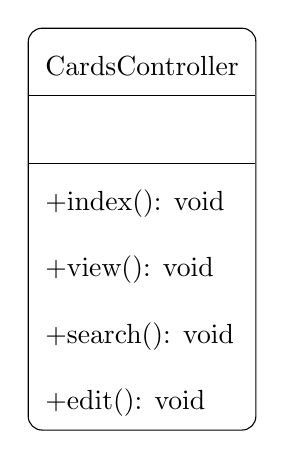
\begin{tikzpicture}
\node (table) [inner sep=0pt] {
\begin{tabular}{l}
  {CardsController} \\
  \hline
  \\
  \hline
  +index(): void \\
  +view(): void \\
  +search(): void \\
  +edit(): void \\
\end{tabular}
};
\draw [rounded corners=.5em] (table.north west) rectangle (table.south east);
\end{tikzpicture}
\caption{Controller:CardsController}
\end{table}

\paragraph{Validazione PadovaCard}
La view collegata ad index corrisponde a quella in figura \ref{validazionecodicebarre}, e permette all'utente di inserire il codice a barre della PadovaCard, manualmente o tramite il lettore.
Il controller index() prende tale valore e recupera le relative informazioni dal database, per poi mostrarle nella view relativa al metodo view. Le informazioni riportate sono:
\begin{itemize}
\item Nome e cognome del possessore della PadovaCard;
\item Data di inizio e fine validità della PadovaCard;
\item Data e ora della visita alla \cappella se si tratta del relativo personale;
\item Validità dell'ingresso, basandosi sul flag "visitato";
\item Se la visita è già stata effettuata, data e ora di tale visita.
\end{itemize}
Dopo aver recuperato le informazioni dal database imposta il flag visitato ad 1, impedendo un ulteriore visita a tale struttura.\\

Si è voluto rendere il più specifici possibile gli errori che la validazione della PadovaCard ritorna, per permettere al personale delle strutture di precisare il motivo per cui l'utente non può visitare la struttura. I possibili errori sono:
\begin{itemize}
\item \textbf{Struttura già visitata}, l'utente cerca di visitare due volte la stessa struttura;
\item \textbf{PadovaCard non attiva}, la PadovaCard è stata disattivata per un qualche motivo che però non è salvato a sistema;
\item \textbf{Struttura non prevista nel pacchetto}, l'utente si reca in una struttura che non fa parte del pacchetto acquistato;
\item \textbf{Data non valida}, l'utente si reca alla struttura in una data al di fuori del range di validità della PadovaCard;
\item \textbf{PadovaCard non valida}, il codice inserito non appartiene a nessuna PadovaCard presente a sistema;
\item \textbf{Leggere l'altro codice}, il codice inserito non è quello della PadovaCard ma quello \tlite, valido solo per la \cappella.
\end{itemize}

\paragrafo{Diagrammi delle attività}
Di seguito è presentato il diagramma delle attività riguardante il processo di verifica di validità di una PadovaCard da parte del personale delle strutture.

\begin{figure}[H]
\centering
\includegraphics[width=0.6\textwidth]{images/validazione_padovacard.png}
\caption{Processo di verifica della validità della PadovaCard}
\end{figure}


\paragrafo{Mokup View}
Di seguito un mockup delle due viste che ha il personale per validare una PadovaCard. Sarà inserito anche un breve tutorial su come leggere le informazioni riportate sulla PadovaCard e su come utilizzare il lettore di codice a barre. Il risultato della lettura sarà mostrato nella stessa pagina, senza bisogno di refresh.
Notare che il focus per la lettura del codice a barre è già sulla casella di input. \\

Questi accorgimenti mirano a semplificare l'interfaccia il più possibile, e a diminuire il numero di click necessari ad operazione, questo perchè molti degli operatori presenti nelle strutture convenzionate sono anziani volontari o membri di categorie protette, che in entrambi i casi non hanno alcuna famigliarità con il computer.
Con gli adattementi descritti un operatore dovrà solamente inserire nome utente e password quindi scansionare con il lettore le PadovaCard, senza toccare mouse o tastiera.
\begin{figure}[H]
\centering
\includegraphics[width=0.5\textwidth]{images/mockup_leggi_barcode.png}
\caption{Schermata per la validazione del codice a barre\label{validazionecodicebarre}}
\end{figure}

\begin{figure}[H]
\centering
\includegraphics[width=0.5\textwidth]{images/mockup_leggi_barcode2.png}
\caption{Risultato validazione}
\end{figure}


\paragraph{Ricerca/Modifica/Stampa PadovaCard}

Le PadovaCard possono essere ricercate utilizzando il loro codice il nominativo del possessore o quello di chi ha effettuato l'ordine. Una volta recuperata una PadovaCard posso modificarla o visualizzare il dettaglio dell'ordine ia cui appartiene e quindi stamparla. \\

Una volta venduta una PadovaCard si possono compiere solo modifiche che non causano una variazione del suo prezzo. Le modifiche possibili sono dunque:
\begin{itemize}
\item Nominativo del possessore, se la ricerca non è stata fatta col nominativo di chi ha effettuato l'ordine;
\item Data/ora di inizio validità;
\item Codice \tlite solo se già presente, non è quindi possibile aggiungerlo o toglierlo.
\end{itemize}
Per quanto riguarda il codice \tlite, se viene modificato sarà l'operatore a dover andare sul software \tlite, annullare la prenotazione relativa al vecchio codice ed effettuarne una nuova per ottenere il nuovo codice. \\

Nel caso in cui la ricerca sia stata fatta con il nominativo di chi ha fatto l'ordine potrò modificare solo la data/ora di inizio validità, ma non per la singola carta, bensì per tutte le carte. Questo per facilitare un cambio di data nel caso di ordini di molte carte (gruppi, scolaresche etc.). \\

Una PadovaCard può essere stampata solamente agli sportelli IAT, in due occasioni:
\begin{enumerate}
\item L'utente è in possesso del voucher, cartaceo o digitale, ma desidera avere la tessera in cartocnino;
\item L'utente ha smarrito la propria PadovaCard e non è in possesso del voucher, si tratta di un caso meno probabile del precedente.
\end{enumerate}
Nel primo caso all'operatore dello IAT basterà utilizzare il lettore dei codice a barre sul codice del voucher per recuperare i dati, quindi avviare la stampa. \\

Il recupero di una PadovaCard smarrita avviene invece tramite nominativo, per cui l'utente dovrà esibire un documento di riconoscimento all'operatore IAT, il quale recupererà i dati tramite nome e cognome, quindi avvierà la stampa. \\	

La stampa è un semplice bottone che avvia in stampa una PadovaCard sull'apposita stampante.

\paragrafo{Mokup View}
Di seguito un mockup della vista che utilizza l'operatore per la ricerca di una PadovaCard.
\begin{figure}[H]
\centering
\includegraphics[width=0.7\textwidth]{images/mockup_stampa_tessera.png}
\caption{Schermata per la ricerca di una PadovaCard\label{stampaPadovaCard}}
\end{figure}

Nell'immagine seguente si vede un mockup della vista per la visualizzazione dei risultati, nella parte superiore può apparire un elenco di PadovaCard tra cui scegliere nel caso in cui la ricerca venga fatta tramite nominativo, e siano presenti più carte appartenenti allo stesso nominativo. Nel caso in cui la ricerca venga fatta tramite intestatario e tale persona ha più ordini salvati nel sistema, si potrà scegliere quale ordine modificare.

\begin{figure}[H]
\centering
\includegraphics[width=0.7\textwidth]{images/mockup_dettagli_ricerca.png}
\caption{Schermata per visualizzare i dettagli di una ricerca}
\end{figure}

\paragrafo{Diagrammi delle attività}
Di seguito è presentato il diagramma delle attività riguardante il processo di modifica della data di validità e del nominativo associati ad una PadovaCard.
\begin{figure}[H]
\centering
\includegraphics[width=1\textwidth]{images/modifica_padovacard.png}
\caption{Processo di modifica dati PadovaCard}
\end{figure}

\subsubsection{Gestione bonifici}
Acquistando tramite call center è possibile effettuare il pagamento via bonifico.
La procedura d'acquisto della PadovaCard rimane uguale a quanto descritto nella Sezione \ref{tdocumentos} e quando si seleziona pagamento tramite bonifico il cliente riceve un email dove vengono specificati conto corrente, causale e importo da versare. Il cliente ha due giorni per effettuare il bonifico e confermare il versamento via email. Gli operatori controlleranno quindi l'estratto conto e in caso positivo concluderanno la vendita e il cliente riceverà i voucher. \\

Oltre all'email con i dati per il pagamento è necessario realizzare un interfaccia che permetta agli operatori di vedere i pagamenti in sospeso e di concluderli. L'index di Tdocumentos mostra già i propri ordini, sia chiusi che pendenti, ma in questo caso ogni operatore ha la necessità di vedere gli ordini di tutti gli operatori in quanto chi effettua l'ordine non è necessariamente colui che lo conclude. Per questo si è deciso di creare una nuova vista dove sono elencati solo i pagamenti via bonifico in attesa di conferma. Per confermare un pagamento si entrerà tramite link alla view dei dettagli dell'ordine. Gli ordini scaduti verranno eliminati.

\paragrafo{Mokup View}
Nell'immagine seguente si vede un mockup della schermata che visualizza i risultati ritornati da una ricerca.

\begin{figure}[H]
\centering
\includegraphics[width=0.7\textwidth]{images/mockup_vista_bonifico.png}
\caption{Schermata per visualizzare i dettagli di una ricerca}
\end{figure}


\subsection{Tracciamento requisiti}\label{tracciamento}

\begin{center}
\def\arraystretch{2}
\begin{longtable}{|p{7cm}|p{3cm}|}
\cellcolor[gray]{0.9} \textbf{Componente} & \cellcolor[gray]{0.9} \textbf{Requisiti} \\ \hline
Users & ROP 14 \newline ROP 15 \newline ROP 16 \newline RFP 18 \newline ROO 19 \newline ROO 20 \newline ROO 21 \\ \hline
Tdocumentos & ROU 2 \newline ROU 3 \newline ROU 4 \newline ROU 5 \newline RFU 12 \newline ROO 23 \newline ROO 24 \newline ROS 26 \\ \hline
Cards & ROU 6 \newline ROP 17 \newline ROS 28 \\ \hline
Cards & ROU 7 \\ \hline
Cards & ROO 25 \newline RFO 31 \\ \hline
\caption{Tracciamento componenti - requisiti}
\end{longtable}

\def\arraystretch{2}
\begin{longtable}{|p{7cm}|p{3cm}|}
\cellcolor[gray]{0.9} \textbf{Requisito} & \cellcolor[gray]{0.9} \textbf{Componenti} \\ \hline
ROU 1 & \\ \hline
ROU 2 & Tdocumentos \\ \hline
ROU 3 & Tdocumentos \\ \hline
ROU 4 & Tdocumentos \\ \hline
ROU 5 & Tdocumentos \\ \hline
ROU 6 & Cards \\ \hline
ROU 7 & Cards \\ \hline
RFU 8 & \\ \hline
RFU 9 & \\ \hline
RFU 10 & \\ \hline
RFU 11 & \\ \hline
RFU 13 & \\ \hline
ROP 14 & User \\ \hline
ROP 15 & User \\ \hline
ROP 16 & User \\ \hline
ROP 17 & Cards \\ \hline
RFP 18 & User \\ \hline
ROO 19 & User \\ \hline
ROO 20 & User \\ \hline
ROO 21 & User \\ \hline
ROO 22 & \tlite \\ \hline
ROO 23 & Tdocumentos \\ \hline
ROO 24 & Tdocumentos \\ \hline
ROO 25 & Cards \\ \hline
ROS 26 & Tdocumentos \\ \hline
ROS 27 & \\ \hline
ROS 28 & Cards \\ \hline
ROS 29 & \\ \hline
RFS 30 & \\ \hline
RFO 31 & Cards \\ \hline
\caption{Tracciamento requisiti - componenti}
\end{longtable}

\end{center} 
